

\section{Introduction} 
% Description of your question(s) Why they are important
\subsection{Why we choose to mine the technologist data}
 It is no secret that the new competition for this century is the 'hunt' for talents., "by 2030, more than 85 million jobs could go unfilled because there are not enough skilled people to take them, according to the latest study conducted by Korn Ferry."\footnote{ \url{https://www.kornferry.com/insights/this-week-in-leadership/talent-crunch-future-of-work}} "The shortage has been amplified by an insufficient number of U.S.-citizen computer science college graduates, restrictive (until recently) and limited H-1B visas for experienced IT professionals to fill the immediate gaps",  echoed the Tech Serve consulting. \footnote{ \url{https://www.techservealliance.org/news/the-state-of-the-technology-talent-shortage/}}
Dice.com's internal analysis already showed that we are going through technology workers (Technologists) shortage, and that is not due to the 'Great Resignation' but due to market demand. Our report will mine through the US H1B data set along with Dice.com's job and candidate profiles (along with skill sets for each job title),  to better understand which technologist job (e.g.: Software developer, Data scientist) are in increasing/decreasing demands, which skill sets (e.g.: Python, C++ etc.) are more popular/unpupular, through time-series. Our goal is to better understand the US technology market and what we can do to help people who try to get into tech market, by providing them with skill-set guidance along with professional training advice. \\
The motivation for this report came from a conversation with one product manager stating that there are no analysis on technologist supply and demand, even on salary data! The product analysts stated they don't have the data, and the R$\&$D team think it is a analyst job and should not 'waste' time on.  I decided to try that as a personal project. As I dive in more, I realized the official data set provided from department of labor is vague and uninformative, most of the job titles are lumped together, and focusing only on salary, hence no detailed information based on skills and locations. I then decided to mine other open source data, while adding relative skill set by mining separate job description data set.\\
My philosophy to tackle this problem/project is to use a simple algorithm on multiple complicated sets, and not the other way: some complex algorithms  on a nice set instead. Personally, I had some 'fatigue' issues with words like 'Deep' and 'Neural' for now, both at work and school, so I've decided to do some old fashion mining by not using heavy GPU computing with 'sexy' machine learning titles, and just have some miner's fun with my hardhat and shovel.\footnote{I will leave that to CSCI 5922-Neural Networks and Deep Learning, this fall.}
\subsection{What is  'Technologist'?}
The simplest definition of a technologist is an expert in a particular field of technology. At Dice, we focus more on an employee's job title and summarizing skill sets to define  whether a candidate is  technologist or not. Engineers and applied scientists are definitely in that category, unfortunately, a musician or a cleaning crew are not. Yet, if his/her resume has certain skill sets that can be applied to solve scientific problem. e.g.: programming, algorithms, him/her  may still be considered as a technologist. For bookkeeping purpose, we currently consider 1468 job titles as technologist, for example: Oracle DBA, Ruby Developer, Research Analyst and Systems Engineer. 
\subsection{What is 'Skill set'?}
As the name suggests, it is the skill that associate with job title of a candidate. Although a individual, such as myself, would like to fit everything single skill that she has ever grasped into a resume, we only consider certain words that are associated with the job title.\\
Take Oracle DBA for example, we tried to limit the particular tech words that are relatively 'unique' or necessary for the job function, so it has 'IT management; PL/SQL; SAN; Unix; Statspack; OEM; Performance tuning; Oracle; Oracle database administration; AWR' as its skill sets. Other skills such as excel and word, we do not consider particularly outstanding compare to OEM, in other word: it is a skill everyone has, which makes them less relevant. Other examples are:
\begin{itemize}
	\item Ruby Developer: Software development; React.js; Ruby on Rails; Ruby; JavaScript
		\item Systems Engineer:	Computer networking; Systems engineering; Quality assurance
\end{itemize}
Next, we will introduce the previous work that has been done to 'stem' the skill set for each technologist title.
\section{Previous/Related Work}
I was always interested in  information retrieval  and knowledge graph, this project gives me the perfect opportunity to pursue those.,Before we can join the skill-sets with H1b data, we need to first 'extract' the keywords.  What I did was using POS tagging to set up skill keywords and trained on 10000+  job title data set, so that to get the labeling for new data set working more accurate. Afterward, we clustered multiple job description for certain job titles and found the common  skill words for each job. \\ 
SpaCy's Pipeline component for part-of-speech taggging\footnote{\url {https://spacy.io/api/tagger}} comes in  really handy for the  data preparation. What we did was to manually add a 'Tag' button for SMEs to spot the 'tech' words from our training set in HTML, resembling the following table:
{
	\begin{center}
		\begin{tabular}{| l | l | l | l | l | r| } 
			\hline
			&	Sentence	&	Word	&	Tag	 & POS &	Job description \# \\ \hline
			0	&	1	&	Softwares		&Tech	& NNPS	&description: 1 \\ \hline
			1	&	2	&	SQL	&	Tech	& NNP &	description: 1 \\ \hline
			2	&	3	&	Java	&	Tech & NNPJ	&	description: 1	\\ \hline
			3		&4		&Web	&	Tech	& NNS&	description: 1\\ \hline
			4	&	5	&	Azure		&Tech	& NNP	&description: 1\\ \hline
			\vdots	&		\vdots	&		\vdots		&	\vdots	&	\vdots	&	\vdots\\ \hline
		\end{tabular}
\end{center}}
Once we got enough samples, we apply the Viterbi algo to the future data set and mine the list of words for each job post, we then trim the list to get the overall skill-set for each title, like the following for sample job titles.  

\begin{center}
	\begin{tabular}{ | p{2.5cm} |p{4.5cm} |}
		\hline
		Job & Skills \\ \hline
		Net Application Developer& Microsoft technologies;Software development;C$\#$;HTML;Quality assurance;ASP.NET;Visual Basic .NET;.NET;Agile.\\\hline
		Android Developer	& Software development;Java;Mobile development;Quality assurance;Android development.\\\hline
		\vdots	&	\vdots\\ \hline
	\end{tabular}
\end{center}
Once we got the whole table for all job titles, we are ready for the major task for this project, getting the data, which will be explained in details in the next section.
\section{Data Set}
%Where from
\subsection{U.S. Department of Labor data}
What better resource to go to than the Department of Labor's statistics, After consulting with a product manager who points to the open API  department provided, I decide to mine their data first.  Shockley though, their data does not give any insight on specific job title but a very general one. I've chosen to call the data between year 2010 and 2021 so that to better match with H1b's time series, and here's what we get, after thorough analysis  of 14027 data entries,with total 34 columns:\\
\begin{table}[h!]
	\caption{Deparrtment of  labour data }
	\resizebox{\columnwidth}{!}
	{%
		
		\begin{tabular}{llll}
			\hline
			{} &    count &  unique &                     top \\
			\hline
			occ\_code   &    14027 &    1507 &                 29-2010 \\
			occ\_group  &     9731 &       5 &                detailed \\
			occ\_title  &    14027 &    1272 &  Tour and Travel Guides \\
			group      &       46 &       2 &                   major \\
			tot\_emp    &  14027.0 &  8936.0 &                 11860.0 \\
			annual     &      852 &       1 &                    True \\
			hourly     &       62 &       1 &                    True \\
			year       &  14027.0 &     NaN &                     NaN \\
			area       &   2658.0 &     NaN &                     NaN \\
			area\_title &     2658 &       1 &                    U.S. \\
			prim\_state &     1329 &       1 &                      US \\
			emp\_prse   &  14027.0 &   229.0 &                     0.5 \\
			mean\_prse  &  14027.0 &     NaN &                     NaN \\
			a\_mean     &    14027 &    6155 &                       * \\
			a\_median   &    14027 &    5808 &                       \# \\
			\hline
		\end{tabular}
		
	}
\end{table}

There are 1272 job titles from department of labor open data, among  them, the only code (15-XXXX) that resemble our definition of technologist  is : 
\begin{itemize}
	\item Computer and Mathematical Occupations 15-0000
\end{itemize}
Unfortunately, only 37 of them instead  what we proposed of roughly 1400+ is publicly stored, they are:\\
{ \small
\begin{itemize}
	\item 'Computer and Mathematical Occupations',
	\item	'Computer and Information Research Scientists',
	\item	'Computer Systems Analysts', 'Computer Programmers',
	\item	'Software Developers, Applications',
	\item	'Software Developers, Systems Software', 'Database Administrators',
	\item	'Network and Computer Systems Administrators*',
	\item	'Computer Support Specialists',
	\item	'Information Security Analysts, Web Developers, and Computer Network Architects',
	\item	'Computer Occupations, All Other*', 'Actuaries', 'Mathematicians',
	\item	'Operations Research Analysts', 'Statisticians',
	\item	'Mathematical Technicians',
	\item	'Mathematical Science Occupations, All Other',
	\item	'Computer Occupations', 'Computer and Information Analysts',
	\item	'Information Security Analysts',
	\item	'Software Developers and Programmers', 'Web Developers',
	\item	'Database and Systems Administrators and Network Architects',
	\item	'Network and Computer Systems Administrators',
	\item	'Computer Network Architects', 'Computer User Support Specialists',
	\item	'Computer Network Support Specialists',
	\item	'Miscellaneous Computer Occupations',
	\item	'Computer Occupations, All Other',
	\item	'Mathematical Science Occupations',
	\item	'Miscellaneous Mathematical Science Occupations',
	\item	'Database and Network Administrators and Architects',
	\item	'Database Administrators and Architects',
	\item	'Software and Web Developers, Programmers, and Testers',
	\item	'Software Developers and Software Quality Assurance Analysts and Testers',
	\item	'Web Developers and Digital Interface Designers',
	\item	'Data Scientists and Mathematical Science Occupations, All Other'.
\end{itemize}
}

This dataset does not provide any details on what do these occupations include. We tried some online resources\footnote{\url{https://occupationdata.github.io/apst_mapping.pdf}} (including DoL's own mapping data from 2018\footnote{\url{https://www.bls.gov/soc/2018/home.htm}, only 20+ were able to  matched, that leaves 1380+ unmatched still }) to try mapping the 1400+ tech job into these 37 categories that yields horribly inaccurate result , which mean we either has to add a new attribute by clustering the 1400 into 15, or again write a new scrapper that mines Glassdoor's data (This should not end up being a scrapper project), even that does not guarantee a good  accuracy since all are self-reported, hence  more biased than H1b data. Due to the time limit, we have to reconcile that. \\
Although, the discovery does not mean DoL's data are completely worthless, there are some good insights that confirm our believe that tech talents are in rising demand. Take Figure \ref{dolnumofemployee} for example:
\begin{figure}[h]
	\begin{center}
		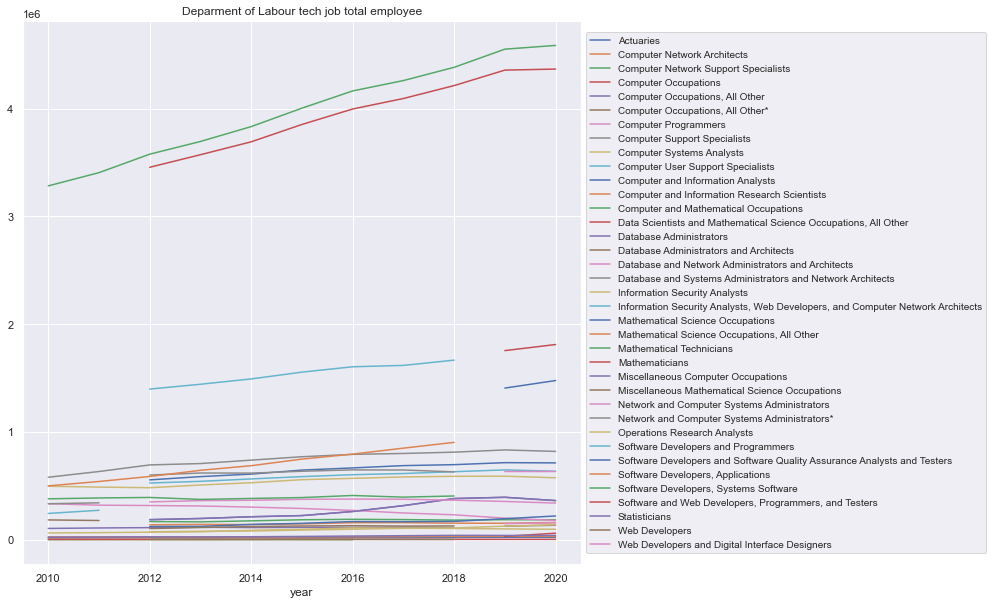
\includegraphics[width=\linewidth]{./photos/totaltech.png}
	\end{center}
	\caption{Deparment of Labour tech jobs number of employee.}
	\label{dolnumofemployee}
	\end{figure}
The top 2 lines represent 'computer occupation' and 'software developer' professions, their growing rates are even higher than the rest of  technologists, it is a clear indication of higher demand for such labor, as opposed to the Farming jobs, which stays relatively the same, in some cases, even declined, as shown in Figure \ref{dolfarming}.
\begin{figure}[h]
	\begin{center}
		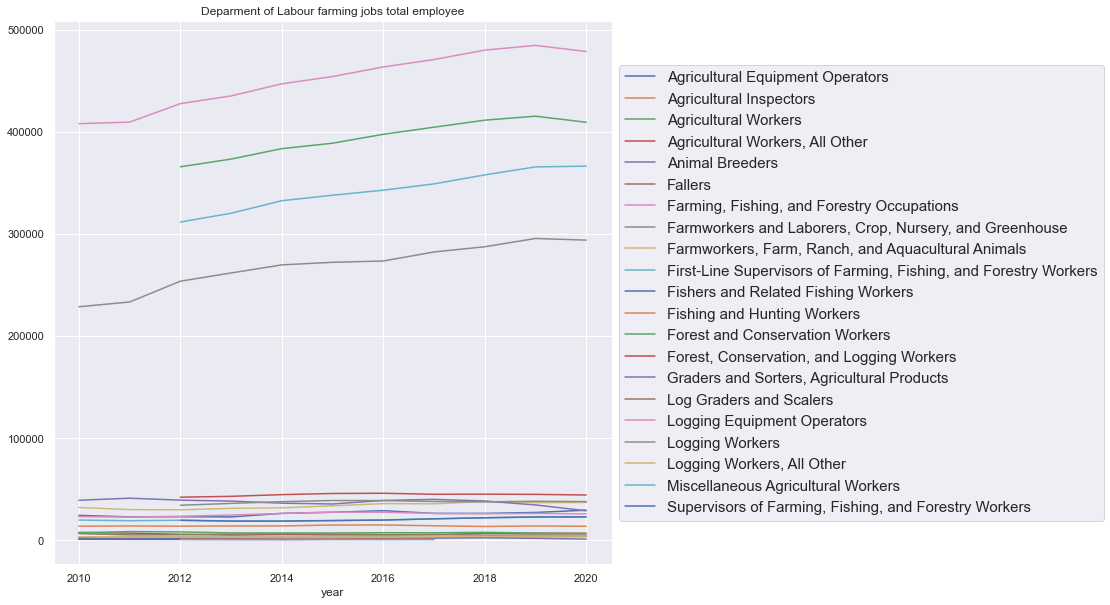
\includegraphics[width=\linewidth]{./photos/dolfarming.png}
	\end{center}
	\caption{Deparment of Labour farming jobs number of employee.}
	\label{dolfarming}
\end{figure}
If we look at the salary data for technologist in Figure \ref{techsalary}, we noticed the significant salary increase over the year, take into account the inflation and supply, it only amply the demand side of the tech market, which forces the employers to hand out competative salary. As oppose farming job market shown in Figure \ref{dolfarmingsalary}, where is did not even cover the inflation over a decade.
\begin{figure}[h]
	\begin{center}
		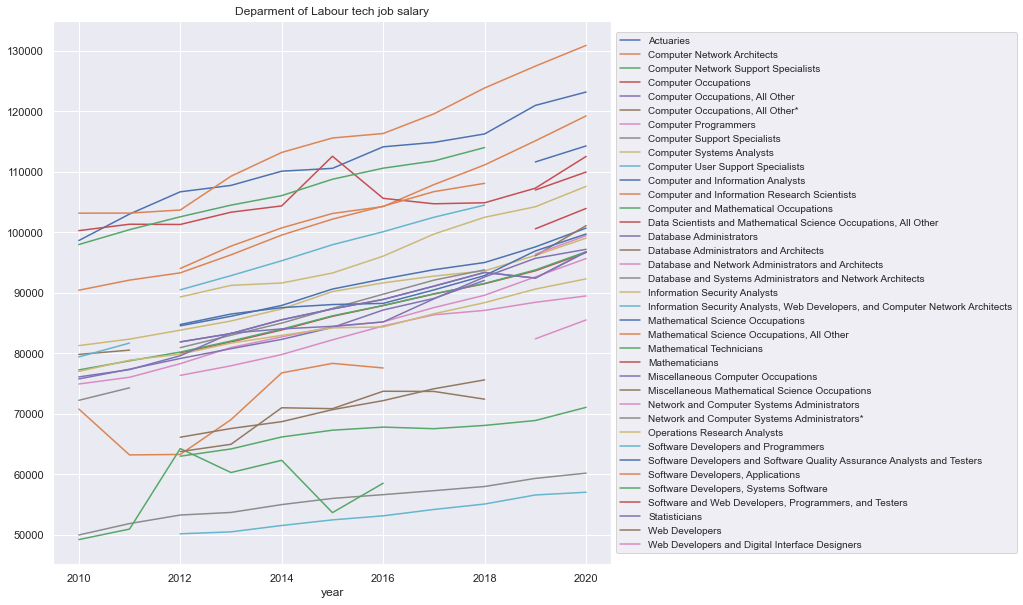
\includegraphics[width=\linewidth]{./photos/departmentoflabour.png}
	\end{center}
	\caption{Deparment of Labour tech job salary.}
	\label{techsalary}
\end{figure}

\begin{figure}[h]
	\begin{center}
		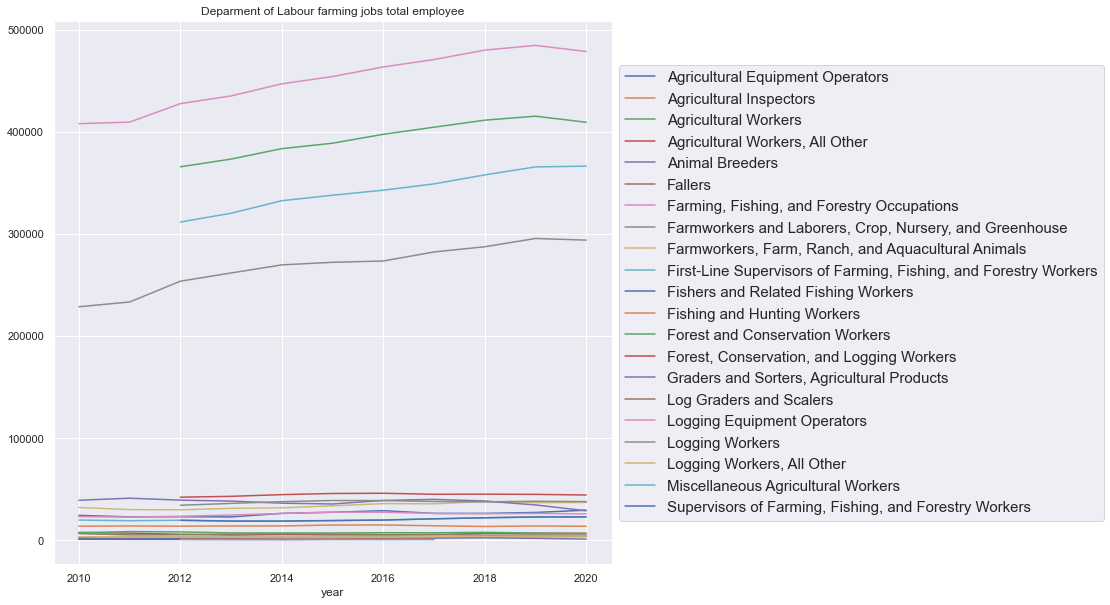
\includegraphics[width=\linewidth]{./photos/dolfarmingsalary.png}
	\end{center}
	\caption{Deparment of Labour farming jobs salary.}
	\label{dolfarmingsalary}
\end{figure}
All of these give us more reasons to find our own data, as an immigrant worker myself, the second 'gold mine' to dig is H1b, which will be the main focus of the next section.
\subsection{H1b data}
 H-1B is a visa in the United States  that allows U.S. employers to temporarily employ foreign workers in specialty occupations (mainly tech). Although, some may argue that "The H-1B temporary visa program has been exploited and abused by employers primarily seeking to fill entry-level positions and reduce overall business costs"\footnote{\url{https://www.uscis.gov}}, that does not necessarily mean these jobs are not in demand, quite the contrary, it is due to market demands. After all, it is not a charity for foreign workers, it is a sign of demand for particular skill-sets here in this country, unfortunately, some company tries to find loopholes in the process. \\
According to H1b law code, the  occupation as requiring theoretical and practical application of a body of "highly specialized knowledge in a field of human endeavor', including but not limited to `biotechnology, chemistry, computing, architecture, engineering, statistics, physical sciences, journalism, medicine and health, economics, education, research, law, accounting, business specialties, technical writing' , and it requires the applicants to have  a bachelor's degree or its equivalent as a minimum to practice in that field. This is a clear indication that it is a technologist candidate, which is another reason I chose such a open source as my project data.\\
We will now move on how to collect such a data from web source.
\subsection{Data scrapping}
Python beautifulsoup is the go-to package for data types of online HTML in my opinion. From the following url link:
{\small \begin{verbatim}
	url = "https://h1bdata.info/index.php?em=&job=%s&city=&year=%d"
\end{verbatim}}
we can tailored the job and city and year as parameters, the HTML table has the following six attributes:
\begin{itemize}
	\item EMPLOYER :  String, Nominal
	\item JOB TITLE :  String, Nominal
	\item BASE SALARY:  Float, Interval
	\item LOCATION:   String,  Nominal
	\item SUBMIT DATE:  (date) String, Ordinal
	\item START DATE:  (date) String, Ordinal
\end{itemize}
We only set the job variable as tech job titles we summarized earlier, and the raw data looks like the following:
% table* stay the same size
	\begin{table}[h]
		\caption{Scrapped data as off July 15th}
		\resizebox{\columnwidth}{!}
		{%
	\begin{tabular}{lllll}
		\hline
		{} &    count & unique &                                                top &    freq \\
		\hline
		Dice\_job\_title &  2495079 &   1180 &                                    Systems Analyst &  198860 \\
		EMPLOYER       &  2495052 &  66795 &                  TATA CONSULTANCY SERVICES LIMITED &  157580 \\
		JOB TITLE      &  2467304 &   1770 &                                    SYSTEMS ANALYST &  198719 \\
		BASE SALARY    &  2467304 &  37871 &                                             60,000 &  146505 \\
		LOCATION       &  2467304 &  10474 &                                       NEW YORK, NY &  136642 \\
		SUBMIT DATE    &  2467304 &   2749 &                                         03/13/2015 &   14268 \\
		START DATE     &  2467304 &   2898 &                                         09/01/2015 &   32532 \\
		Job\_Title      &  2495079 &   1180 &                                    Systems Analyst &  198860 \\
%		relatedSkills  &  2489574 &   1101 &  Software development;Systems analysis;SQL;Qual... &  198860 \\
		\hline
	\end{tabular}
    }
	\end{table}

Next, we will look at the exploratory data analysis.  
\subsection{EDA}
Figure \ref{top10comp} shows the top 10 companies that submit H1b over the year, and we can clearly spot the visa 'abusers'. But what is more interesting is that it has some bit tech company's on the list, I do not consider it as a sign of abuse, due to the 'tech' nature of IBM, Google, and Microsoft, quite the opposite, it re-affirmed  the thesis of this project: tech skills are in high demands. \\
\begin{figure}[h!]
	\begin{center}
		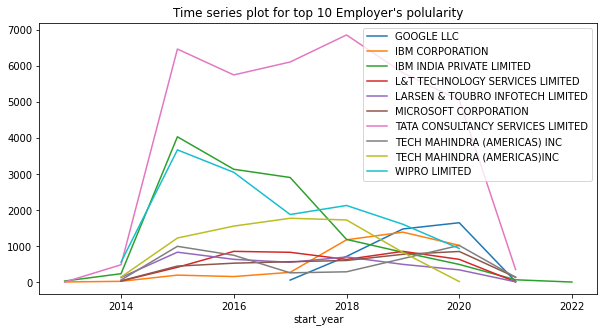
\includegraphics[width=\linewidth]{./photos/top10employers_timeseries.png}
	\end{center}
	\caption{Top 10 companies filing H1b visa.}
	\label{top10comp}
\end{figure}
Figure \ref{top10job} shows that the  top job title filed for the visa, and it is clearly the `trendy' titles.  \\
\begin{figure}[h!]
	\begin{center}
		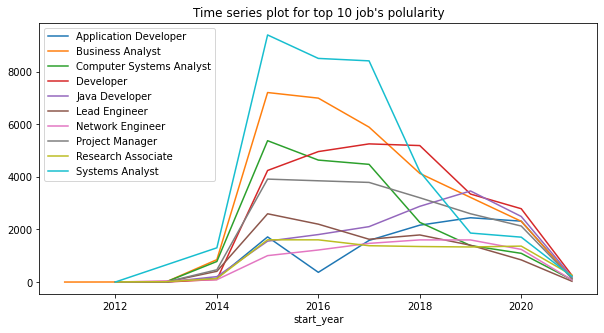
\includegraphics[width=\linewidth]{./photos/top10job_timeseries.png}
	\end{center}
	\caption{Top 10 job applied for H1b visa over 10 year period.}
	\label{top10job}
\end{figure}
Figure \ref{top10state} indicated the states that have the most H1b submission, not very far from the talent pools. \\
\begin{figure}[h!]
	\begin{center}
		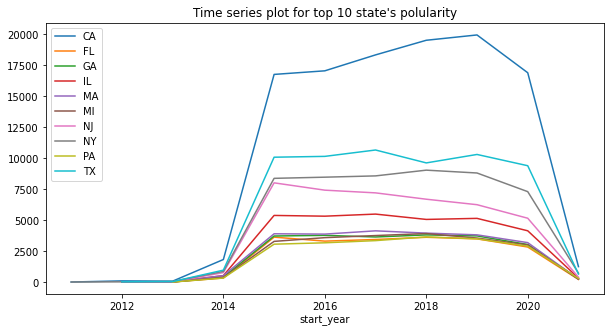
\includegraphics[width=\linewidth]{./photos/top10state_timeseries.png}
	\end{center}
	\caption{Top 10 states filed for H1b visa.}
	\label{top10state}
\end{figure}
Two more information we can read from these plotting. First, it is a clear indication that after 2016 elections, there are some declined on H1b application due to policies. Second, the outlier data between year 2012 to  2014, and again from year 2020 to 2021. Shows that we do not have enough data on those particular years, and not because the titles are dying. If we focus only on year between 2015 to 2019 and do linear regression, we can easily see the demands should in fact go up. \\
Last but not the least, the salary data from Figure \ref{top10jobbox} and Figure \ref{top10statebox} may help us understand where are the talents needed and preferable jobs that are out there. 
\begin{figure}[h!]
	\begin{center}
		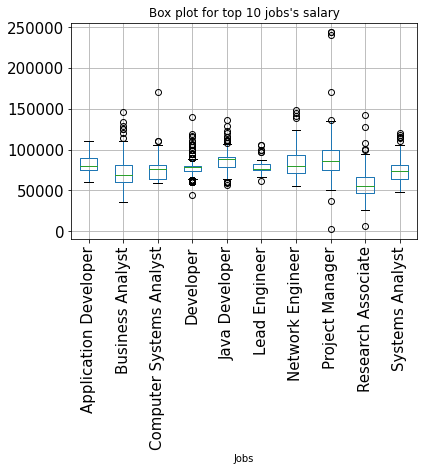
\includegraphics[width=\linewidth]{./photos/top10jobs.png}
	\end{center}
	\caption{Top 10 job salary box plot.}
	\label{top10jobbox}
\end{figure}
\begin{figure}[h!]
	\begin{center}
		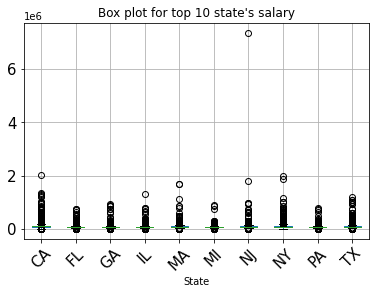
\includegraphics[width=\linewidth]{./photos/top10state.png}
	\end{center}
	\caption{Top 10 state salary box plot.}
	\label{top10statebox}
\end{figure}
In addition, we can spot some of the lest popular job titles associated with H1b application as in Table \ref{leastpopularjob}
	\begin{table}[h]
	\caption{Least 'popular' technologist job titles in  H1b data}
	\label{leastpopularjob}
	\resizebox{\columnwidth}{!}
	{%
	\begin{tabular}{ll}
		\hline
		{} &                    Dice\_job\_title \\
		\hline
		300  &       Dynamics Functional Analyst \\
		282  &           Director Infrastructure \\
		354  &                      F\# Developer \\
		1076 &  Vulnerability Management Analyst \\
		1067 &                       Vertica DBA \\
		63   &                    Avaya Engineer \\
		255  &           Desktop Support Analyst \\
		291  &      Disaster Recovery Specialist \\
		345  &                   Epic Consultant \\
		\hline
	\end{tabular}
	}
\end{table}
The least popular states as shown in Figure \ref{leastpopular}. \\
\begin{figure}[h]
	
	\centering
	\begin{minipage}{.48\linewidth}
		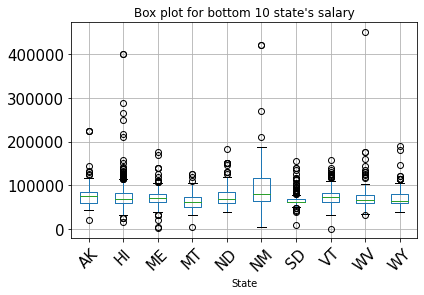
\includegraphics[width=\linewidth]{./photos/bottom10statebox.png}


	\end{minipage}
	\hfill
	\begin{minipage}{.48\linewidth}
		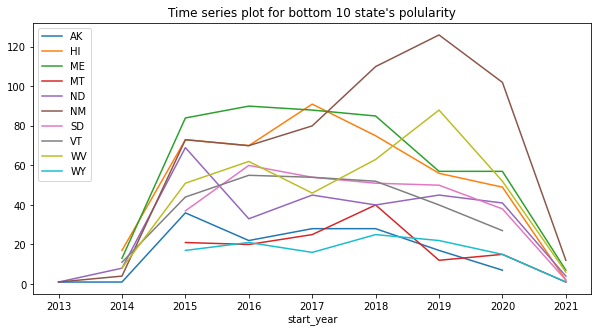
\includegraphics[width=\linewidth]{./photos/bottom10statetime.png}


	\end{minipage}
\caption{Bottom 10 states for hiring tech talents.}
\label{leastpopular}
\end{figure}

\section{Main Techniques Applied}
%Data clean/preprocess/etc.
%Data Warehouse/cube/etc.
%Classification/Clustering/etc.
Once we are  done with  data scrapping using beautiful soup and analyzed with pandas along matplotlib. we can move on to the most important part of the project: data cleaning.
\subsection{Data cleaning}
This is by far the most time-consuming process, yet we can not ignore. Duplicity is a tricky concept for this data set, due to the highly likely possibility of a company has multiple submissions on the same day at the same city. Yet, we decided to drop the duplicates, because we believe a single hire is already a strong signal for that particular job title, and we want to avoid the unnecessary noise while clustering. \\
Outlier detection is another process that needed to be carefully orchestrated, not  much so for the job title, but for the salary data. As we already noticed in Figure \ref{top10statebox}, that some of the salaries are just too high for it to be considered worth averaging, we decide to ignore any salary that approximate 1 million, but do little for the lower end of the tile, in order to spot the salary abuse case. In the end, we e ended up having a fewer number of data point(70$\%$ shrinks), as shown in Table \ref{newdata}.
\begin{table}[h!]
	\caption{New h1b data after data cleaning process}
	\label{newdata}
	\resizebox{\columnwidth}{!}
	{%
		
		\begin{tabular}{lllll}
			\hline
			{} &   count & unique &                                                top &   freq \\
			\hline
			Dice\_job\_title &  603967 &   1107 &                                    Systems Analyst &  35605 \\
			EMPLOYER       &  603967 &  66538 &                  TATA CONSULTANCY SERVICES LIMITED &  36885 \\
			JOB TITLE      &  603967 &   1655 &                                    SYSTEMS ANALYST &  35605 \\
			BASE SALARY    &  603967 &  37791 &                                             60,000 &  23256 \\
			LOCATION       &  603967 &  10453 &                                       NEW YORK, NY &  34957 \\
			SUBMIT DATE    &  603967 &   2747 &                                         03/16/2018 &   2377 \\
			START DATE     &  603967 &   2897 &                                         10/01/2020 &  17065 \\
			Job\_Title      &  603967 &   1107 &                                    Systems Analyst &  35605 \\
%			relatedSkills  &  603967 &   1101 &  Software development;Systems analysis;SQL;Qual... &  35605 \\
			\hline
		\end{tabular}
		
	}

\end{table}

\subsection{Data processing and integration}
After cleaning, we can then combine the skill-set data with H1b data, Pandas merge and join function can do the trick (we also need astype method to convert the objects into the right data type, along with splitting the location string and date string to extract the state and city information  for H1b starting year info).
\begin{verbatim}
pd.merge(df_project, jobs, left_on=  ['occ_title'],
right_on= ['Job_Title'], 
how = 'outer')
\end{verbatim}
The data frame in the end would look like:
\begin{table}[h!]
	\caption{Data frame(pandas) for the New h1b with integration on skill sets}
	\resizebox{\columnwidth}{3cm}
	{%
\begin{tabular}{llllllllll}
	
	\hline
	{} &              Dice\_job\_title &                                           EMPLOYER &                   JOB TITLE & BASE SALARY &            LOCATION & SUBMIT DATE &  START DATE &                   Job\_Title &                                      relatedSkills \\
	\hline
	0  &  .Net Application Developer &                                            VCA INC &  .NET APPLICATION DEVELOPER &      80,000 &   SILVER SPRING, MD &  11/24/2014 &  11/28/2014 &  .Net Application Developer &  Microsoft technologies;Software development;C\#... \\
	1  &  .Net Application Developer &                                 OPTUM SERVICES INC &  .NET APPLICATION DEVELOPER &      83,158 &   GOLDEN VALLEY, MN &  12/10/2014 &  12/29/2014 &  .Net Application Developer &  Microsoft technologies;Software development;C\#... \\
	2  &  .Net Application Developer &                                            LCG INC &  .NET APPLICATION DEVELOPER &      89,669 &       ARLINGTON, VA &  12/30/2014 &  01/12/2015 &  .Net Application Developer &  Microsoft technologies;Software development;C\#... \\
	3  &  .Net Application Developer &                                            VCA INC &  .NET APPLICATION DEVELOPER &      80,000 &   SILVER SPRING, MD &  11/24/2014 &  11/28/2014 &  .Net Application Developer &  Microsoft technologies;Software development;C\#... \\
	4  &  .Net Application Developer &                                 OPTUM SERVICES INC &  .NET APPLICATION DEVELOPER &      83,158 &   GOLDEN VALLEY, MN &  12/10/2014 &  12/29/2014 &  .Net Application Developer &  Microsoft technologies;Software development;C\#... \\
	5  &  .Net Application Developer &                                            LCG INC &  .NET APPLICATION DEVELOPER &      89,669 &       ARLINGTON, VA &  12/30/2014 &  01/12/2015 &  .Net Application Developer &  Microsoft technologies;Software development;C\#... \\
	6  &  .Net Application Developer &             MULTITEK SYSTEMS \& DESIGN INCORPORATED &  .NET APPLICATION DEVELOPER &      42,000 &       DEER PARK, NY &  03/14/2015 &  09/12/2015 &  .Net Application Developer &  Microsoft technologies;Software development;C\#... \\
	7  &  .Net Application Developer &                          CNET GLOBAL SOLUTIONS INC &  .NET APPLICATION DEVELOPER &      60,600 &       WATERTOWN, MA &  08/26/2015 &  09/04/2015 &  .Net Application Developer &  Microsoft technologies;Software development;C\#... \\
	8  &  .Net Application Developer &                                      NET TANGO INC &  .NET APPLICATION DEVELOPER &      61,800 &      LOUISVILLE, KY &  02/23/2015 &  08/22/2015 &  .Net Application Developer &  Microsoft technologies;Software development;C\#... \\
	9  &  .Net Application Developer &                            VEDICSOFT SOLUTIONS LLC &  .NET APPLICATION DEVELOPER &      73,445 &        NEW YORK, NY &  06/26/2015 &  07/13/2015 &  .Net Application Developer &  Microsoft technologies;Software development;C\#... \\
	10 &  .Net Application Developer &  NATIONAL COUNCIL OF YMCAS OF THE UNITED STATES... &  .NET APPLICATION DEVELOPER &      85,000 &         CHICAGO, IL &  10/22/2015 &  12/01/2015 &  .Net Application Developer &  Microsoft technologies;Software development;C\#... \\
	11 &  .Net Application Developer &                   MERIDIAN KNOWLEDGE SOLUTIONS LLC &  .NET APPLICATION DEVELOPER &      95,000 &         HERNDON, VA &  06/27/2015 &  07/06/2015 &  .Net Application Developer &  Microsoft technologies;Software development;C\#... \\
	12 &  .Net Application Developer &                   MERIDIAN KNOWLEDGE SOLUTIONS LLC &  .NET APPLICATION DEVELOPER &      95,000 &         HERNDON, VA &  06/30/2015 &  07/06/2015 &  .Net Application Developer &  Microsoft technologies;Software development;C\#... \\
	13 &  .Net Application Developer &                       MERIDIAN KNOWLEDGE SOLUTIONS &  .NET APPLICATION DEVELOPER &      95,000 &          RESTON, VA &  07/17/2015 &  07/28/2015 &  .Net Application Developer &  Microsoft technologies;Software development;C\#... \\
	14 &  .Net Application Developer &                  SONY DADC NEW MEDIA SOLUTIONS INC &  .NET APPLICATION DEVELOPER &      99,798 &  MARINA DEL REY, CA &  06/22/2015 &  06/22/2015 &  .Net Application Developer &  Microsoft technologies;Software development;C\#... \\
	15 &  .Net Application Developer &                                            VCA INC &  .NET APPLICATION DEVELOPER &      80,000 &   SILVER SPRING, MD &  11/24/2014 &  11/28/2014 &  .Net Application Developer &  Microsoft technologies;Software development;C\#... \\
	16 &  .Net Application Developer &                                 OPTUM SERVICES INC &  .NET APPLICATION DEVELOPER &      83,158 &   GOLDEN VALLEY, MN &  12/10/2014 &  12/29/2014 &  .Net Application Developer &  Microsoft technologies;Software development;C\#... \\
	17 &  .Net Application Developer &                                            LCG INC &  .NET APPLICATION DEVELOPER &      89,669 &       ARLINGTON, VA &  12/30/2014 &  01/12/2015 &  .Net Application Developer &  Microsoft technologies;Software development;C\#... \\
	18 &  .Net Application Developer &             MULTITEK SYSTEMS \& DESIGN INCORPORATED &  .NET APPLICATION DEVELOPER &      42,000 &       DEER PARK, NY &  03/14/2015 &  09/12/2015 &  .Net Application Developer &  Microsoft technologies;Software development;C\#... \\
	19 &  .Net Application Developer &                          CNET GLOBAL SOLUTIONS INC &  .NET APPLICATION DEVELOPER &      60,600 &       WATERTOWN, MA &  08/26/2015 &  09/04/2015 &  .Net Application Developer &  Microsoft technologies;Software development;C\#... \\
	20 &  .Net Application Developer &                                      NET TANGO INC &  .NET APPLICATION DEVELOPER &      61,800 &      LOUISVILLE, KY &  02/23/2015 &  08/22/2015 &  .Net Application Developer &  Microsoft technologies;Software development;C\#... \\
	21 &  .Net Application Developer &                            VEDICSOFT SOLUTIONS LLC &  .NET APPLICATION DEVELOPER &      73,445 &        NEW YORK, NY &  06/26/2015 &  07/13/2015 &  .Net Application Developer &  Microsoft technologies;Software development;C\#... \\
	22 &  .Net Application Developer &  NATIONAL COUNCIL OF YMCAS OF THE UNITED STATES... &  .NET APPLICATION DEVELOPER &      85,000 &         CHICAGO, IL &  10/22/2015 &  12/01/2015 &  .Net Application Developer &  Microsoft technologies;Software development;C\#... \\
	23 &  .Net Application Developer &                   MERIDIAN KNOWLEDGE SOLUTIONS LLC &  .NET APPLICATION DEVELOPER &      95,000 &         HERNDON, VA &  06/27/2015 &  07/06/2015 &  .Net Application Developer &  Microsoft technologies;Software development;C\#... \\
	24 &  .Net Application Developer &                   MERIDIAN KNOWLEDGE SOLUTIONS LLC &  .NET APPLICATION DEVELOPER &      95,000 &         HERNDON, VA &  06/30/2015 &  07/06/2015 &  .Net Application Developer &  Microsoft technologies;Software development;C\#... \\
	25 &  .Net Application Developer &                       MERIDIAN KNOWLEDGE SOLUTIONS &  .NET APPLICATION DEVELOPER &      95,000 &          RESTON, VA &  07/17/2015 &  07/28/2015 &  .Net Application Developer &  Microsoft technologies;Software development;C\#... \\
	26 &  .Net Application Developer &                  SONY DADC NEW MEDIA SOLUTIONS INC &  .NET APPLICATION DEVELOPER &      99,798 &  MARINA DEL REY, CA &  06/22/2015 &  06/22/2015 &  .Net Application Developer &  Microsoft technologies;Software development;C\#... \\
	27 &  .Net Application Developer &                                ZENTEK INFOSOFT INC &  .NET APPLICATION DEVELOPER &      94,000 &        BROOKLYN, NY &  04/16/2016 &  04/18/2016 &  .Net Application Developer &  Microsoft technologies;Software development;C\#... \\
	28 &  .Net Application Developer &                            VEDICSOFT SOLUTIONS LLC &  .NET APPLICATION DEVELOPER &      73,445 &        NEW YORK, NY &  05/03/2016 &  11/01/2016 &  .Net Application Developer &  Microsoft technologies;Software development;C\#... \\
	29 &  .Net Application Developer &                       DOYEN BUSINESS SOLUTIONS INC &  .NET APPLICATION DEVELOPER &      76,000 &         ATLANTA, GA &  02/02/2016 &  02/09/2016 &  .Net Application Developer &  Microsoft technologies;Software development;C\#... \\
	30 &  .Net Application Developer &                                   ACI INFOTECH INC &  .NET APPLICATION DEVELOPER &      80,000 &      PISCATAWAY, NJ &  02/24/2016 &  08/25/2016 &  .Net Application Developer &  Microsoft technologies;Software development;C\#... \\
	31 &  .Net Application Developer &                 ANALYSTS INTERNATIONAL CORPORATION &  .NET APPLICATION DEVELOPER &      91,541 &          ITASCA, IL &  08/17/2016 &  08/25/2016 &  .Net Application Developer &  Microsoft technologies;Software development;C\#... \\
	32 &  .Net Application Developer &            AMERICAN SOCIETY FOR RADIATION ONCOLOGY &  .NET APPLICATION DEVELOPER &      92,000 &       ARLINGTON, VA &  07/18/2016 &  07/25/2016 &  .Net Application Developer &  Microsoft technologies;Software development;C\#... \\
	33 &  .Net Application Developer &                                ZENTEK INFOSOFT INC &  .NET APPLICATION DEVELOPER &     100,000 &        BROOKLYN, NY &  04/16/2016 &  04/18/2016 &  .Net Application Developer &  Microsoft technologies;Software development;C\#... \\
	34 &  .Net Application Developer &                             RANGAM CONSULTANTS INC &  .NET APPLICATION DEVELOPER &     114,400 &        NEW YORK, NY &  09/30/2016 &  03/27/2017 &  .Net Application Developer &  Microsoft technologies;Software development;C\#... \\
	35 &  .Net Application Developer &                             RANGAM CONSULTANTS INC &  .NET APPLICATION DEVELOPER &     114,400 &        NEW YORK, NY &  09/30/2016 &  03/27/2017 &  .Net Application Developer &  Microsoft technologies;Software development;C\#... \\
	36 &  .Net Application Developer &                                            VCA INC &  .NET APPLICATION DEVELOPER &      80,000 &   SILVER SPRING, MD &  11/24/2014 &  11/28/2014 &  .Net Application Developer &  Microsoft technologies;Software development;C\#... \\
	37 &  .Net Application Developer &                                 OPTUM SERVICES INC &  .NET APPLICATION DEVELOPER &      83,158 &   GOLDEN VALLEY, MN &  12/10/2014 &  12/29/2014 &  .Net Application Developer &  Microsoft technologies;Software development;C\#... \\
	38 &  .Net Application Developer &                                            LCG INC &  .NET APPLICATION DEVELOPER &      89,669 &       ARLINGTON, VA &  12/30/2014 &  01/12/2015 &  .Net Application Developer &  Microsoft technologies;Software development;C\#... \\
	39 &  .Net Application Developer &             MULTITEK SYSTEMS \& DESIGN INCORPORATED &  .NET APPLICATION DEVELOPER &      42,000 &       DEER PARK, NY &  03/14/2015 &  09/12/2015 &  .Net Application Developer &  Microsoft technologies;Software development;C\#... \\
	40 &  .Net Application Developer &                          CNET GLOBAL SOLUTIONS INC &  .NET APPLICATION DEVELOPER &      60,600 &       WATERTOWN, MA &  08/26/2015 &  09/04/2015 &  .Net Application Developer &  Microsoft technologies;Software development;C\#... \\
	41 &  .Net Application Developer &                                      NET TANGO INC &  .NET APPLICATION DEVELOPER &      61,800 &      LOUISVILLE, KY &  02/23/2015 &  08/22/2015 &  .Net Application Developer &  Microsoft technologies;Software development;C\#... \\
	42 &  .Net Application Developer &                            VEDICSOFT SOLUTIONS LLC &  .NET APPLICATION DEVELOPER &      73,445 &        NEW YORK, NY &  06/26/2015 &  07/13/2015 &  .Net Application Developer &  Microsoft technologies;Software development;C\#... \\
	43 &  .Net Application Developer &  NATIONAL COUNCIL OF YMCAS OF THE UNITED STATES... &  .NET APPLICATION DEVELOPER &      85,000 &         CHICAGO, IL &  10/22/2015 &  12/01/2015 &  .Net Application Developer &  Microsoft technologies;Software development;C\#... \\
	44 &  .Net Application Developer &                   MERIDIAN KNOWLEDGE SOLUTIONS LLC &  .NET APPLICATION DEVELOPER &      95,000 &         HERNDON, VA &  06/27/2015 &  07/06/2015 &  .Net Application Developer &  Microsoft technologies;Software development;C\#... \\
	45 &  .Net Application Developer &                   MERIDIAN KNOWLEDGE SOLUTIONS LLC &  .NET APPLICATION DEVELOPER &      95,000 &         HERNDON, VA &  06/30/2015 &  07/06/2015 &  .Net Application Developer &  Microsoft technologies;Software development;C\#... \\
	46 &  .Net Application Developer &                       MERIDIAN KNOWLEDGE SOLUTIONS &  .NET APPLICATION DEVELOPER &      95,000 &          RESTON, VA &  07/17/2015 &  07/28/2015 &  .Net Application Developer &  Microsoft technologies;Software development;C\#... \\
	47 &  .Net Application Developer &                  SONY DADC NEW MEDIA SOLUTIONS INC &  .NET APPLICATION DEVELOPER &      99,798 &  MARINA DEL REY, CA &  06/22/2015 &  06/22/2015 &  .Net Application Developer &  Microsoft technologies;Software development;C\#... \\
	48 &  .Net Application Developer &                                ZENTEK INFOSOFT INC &  .NET APPLICATION DEVELOPER &      94,000 &        BROOKLYN, NY &  04/16/2016 &  04/18/2016 &  .Net Application Developer &  Microsoft technologies;Software development;C\#... \\
	49 &  .Net Application Developer &                            VEDICSOFT SOLUTIONS LLC &  .NET APPLICATION DEVELOPER &      73,445 &        NEW YORK, NY &  05/03/2016 &  11/01/2016 &  .Net Application Developer &  Microsoft technologies;Software development;C\#... \\
	\hline
\end{tabular}
		
	}
	
\end{table}
The reason for that is to associate each title with particular skill set that we clustered in the previous work. Now we are ready to cluster the data we have.
\subsection{Machine learning}
No project seems complete without the magic hand of machine learning nowadays. Although I personally believe we are still at baby stage of vector computing, as Jedea Pearl called it: the first ladder of causality: Association\footnote{The Book of Why: The New Science of Cause and Effect. 2018.}, it i still worth the effort since it suite well with more data collection with better computing resource. Yet, we can not naively think it as a black box just to get the job done, we are at the stage of realizing that iterative methods can only you so far, to qoute François Chollet" "Training ever bigger convnets and LSTMs on ever bigger datasets gets us closer to Strong AI -- in the same sense that building taller towers gets us closer to the moon." Next, we consider a unsupervised learning for the model, since we have no idea which skill-set should go to which cluster.
\subsubsection{K-means}
Word2Vec algorithm is a natural language processing technique invented at Google. It maps words to vectors of real numbers, or in other words, embedding the word into vectors. We would be using sk-learn package mainly, to first vectorize the skill-set string of words, with the help of cluster's \textbf{KMeans} package to cluster the texts. The logic here is use the vector representations of words learned from word2vec, and semantically put similar words close to each other in a 2-D vector space. Using K means algorithm, we then can group words from the text into similar groups and analyze the results.\\
We  use Principal Component Analysis (PCA) for the purpose of  dimensionality reduction, in order to map the work into 2-D space. A example of 5 clusters is shown in Figure \ref{pca} 
\begin{figure}[h]
	\begin{center}
		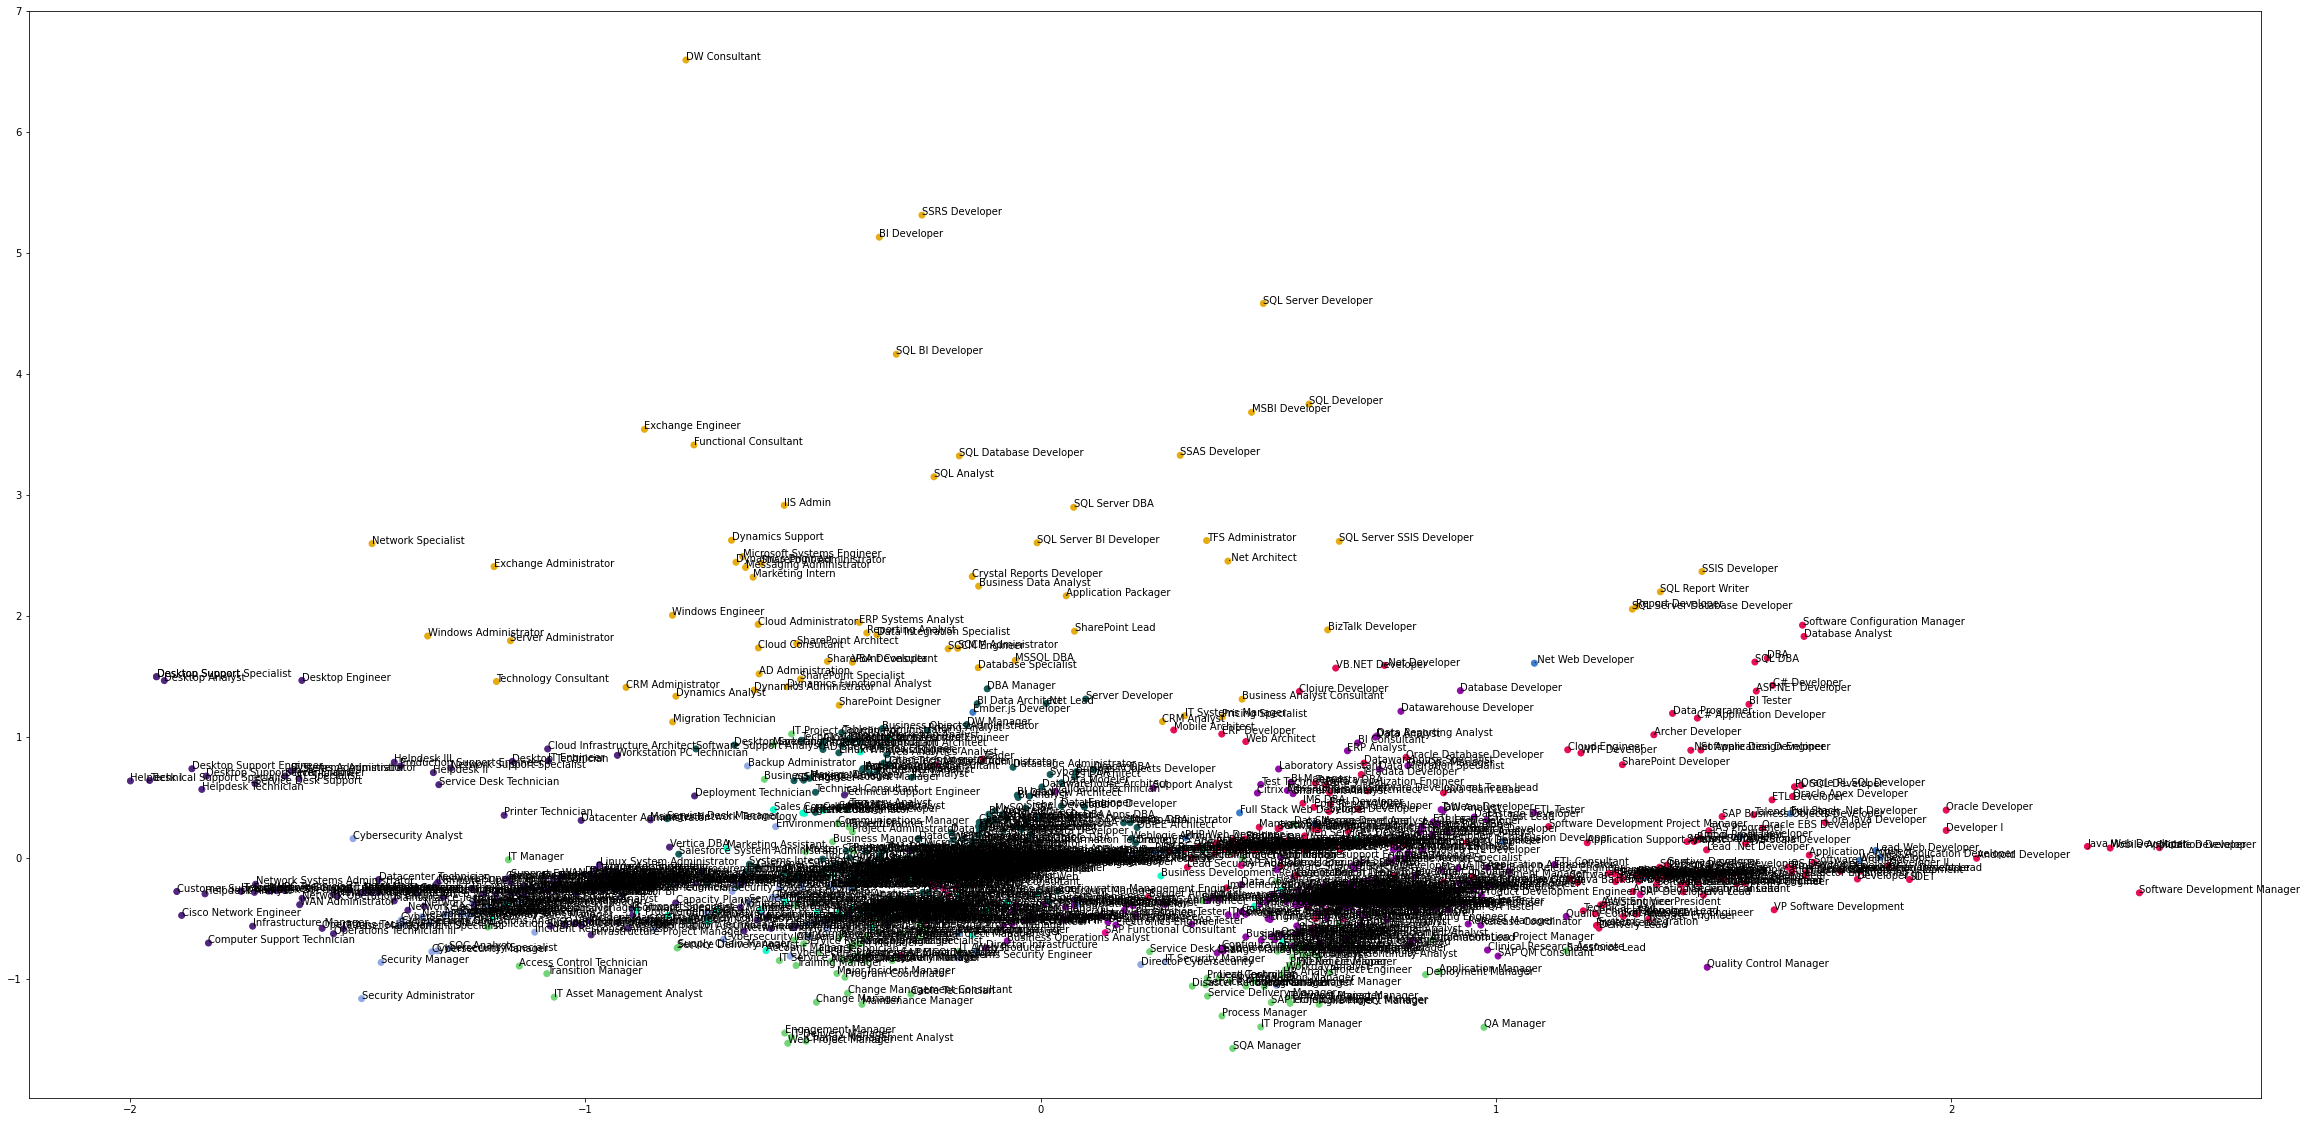
\includegraphics[width=.9\linewidth]{./photos/clusterscatter.png}
	\end{center}
	\caption{Clustering by job skill sets}
	\label{pca}
\end{figure}
\subsubsection{Evaluation of the clustering}
The elbow method helps to choose the optimum value of k by fitting the model with a range of values for the number of clusters. We can consider it as a 'cost'-function, we define it as We defined it  as and $\epsilon$ which is sum of squares  distance between data points and respective centroid of cluster to which the data point belongs, we stop when the $\epsilon$ (iterations) converges. But, as we see in Figure \ref{elbow}, there is no 'optimal' number of neighbor that we can choose from. One of the reasons for that is the tech skills for the job are 'convoluted', meaning the distance between each job title are closer than we first vision. Yet, we can still borrow from department of labor data set when categorizing the tech job titles, and set the k equals to 10.

\begin{figure}[h]
	\begin{center}
		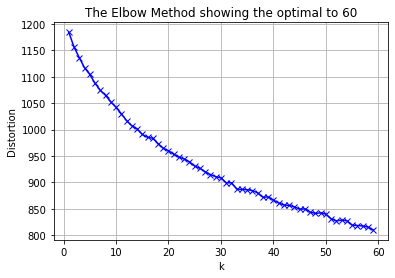
\includegraphics[width=\linewidth]{./photos/elbow.png}
	\end{center}
	\caption{Clustering Elbow method  by job skill sets}
	\label{elbow}
\end{figure}
Training on all H1b data set does not make much difference, as shown in Figure \ref{elbowbig}, it take longer to train while the results are the same, yet the distance are way higher. 
\begin{figure}[h]
	\begin{center}
		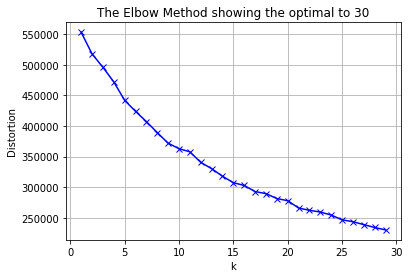
\includegraphics[width=\linewidth]{./photos/elbow for 2mil.png}
	\end{center}
	\caption{Clustering Elbow method using all H1b data}
	\label{elbowbig}
\end{figure}

\section{Key Results}
%What did you discover/learn?
\subsection{Trending Skills}
We successfully  mined the top 10 job titles that are in demand, they are: System analyst, Developer, Business Analyst, Computer System analyst, System Administrator, Project manager, Java Developer, System engineer, Application Developer. Lead Engineer. As opposed to media's champion: Data scientist and ML engineer. Next, we will explore the skill trend. Figure \ref{trending} shows us a clear image of what are the top skill that dominate each year's skill. QA and Software developer ranked 1 and 2 with no decline in sight. System analyst, on the other hand, is  becoming less popular over the year, probably due to job automation, so is SQL. Cloud computing is on the rise, along with agile, it is a clear sign that cloud engineering and project management will be in huge demand in the future. 
\begin{figure}[h]
	\begin{center}
		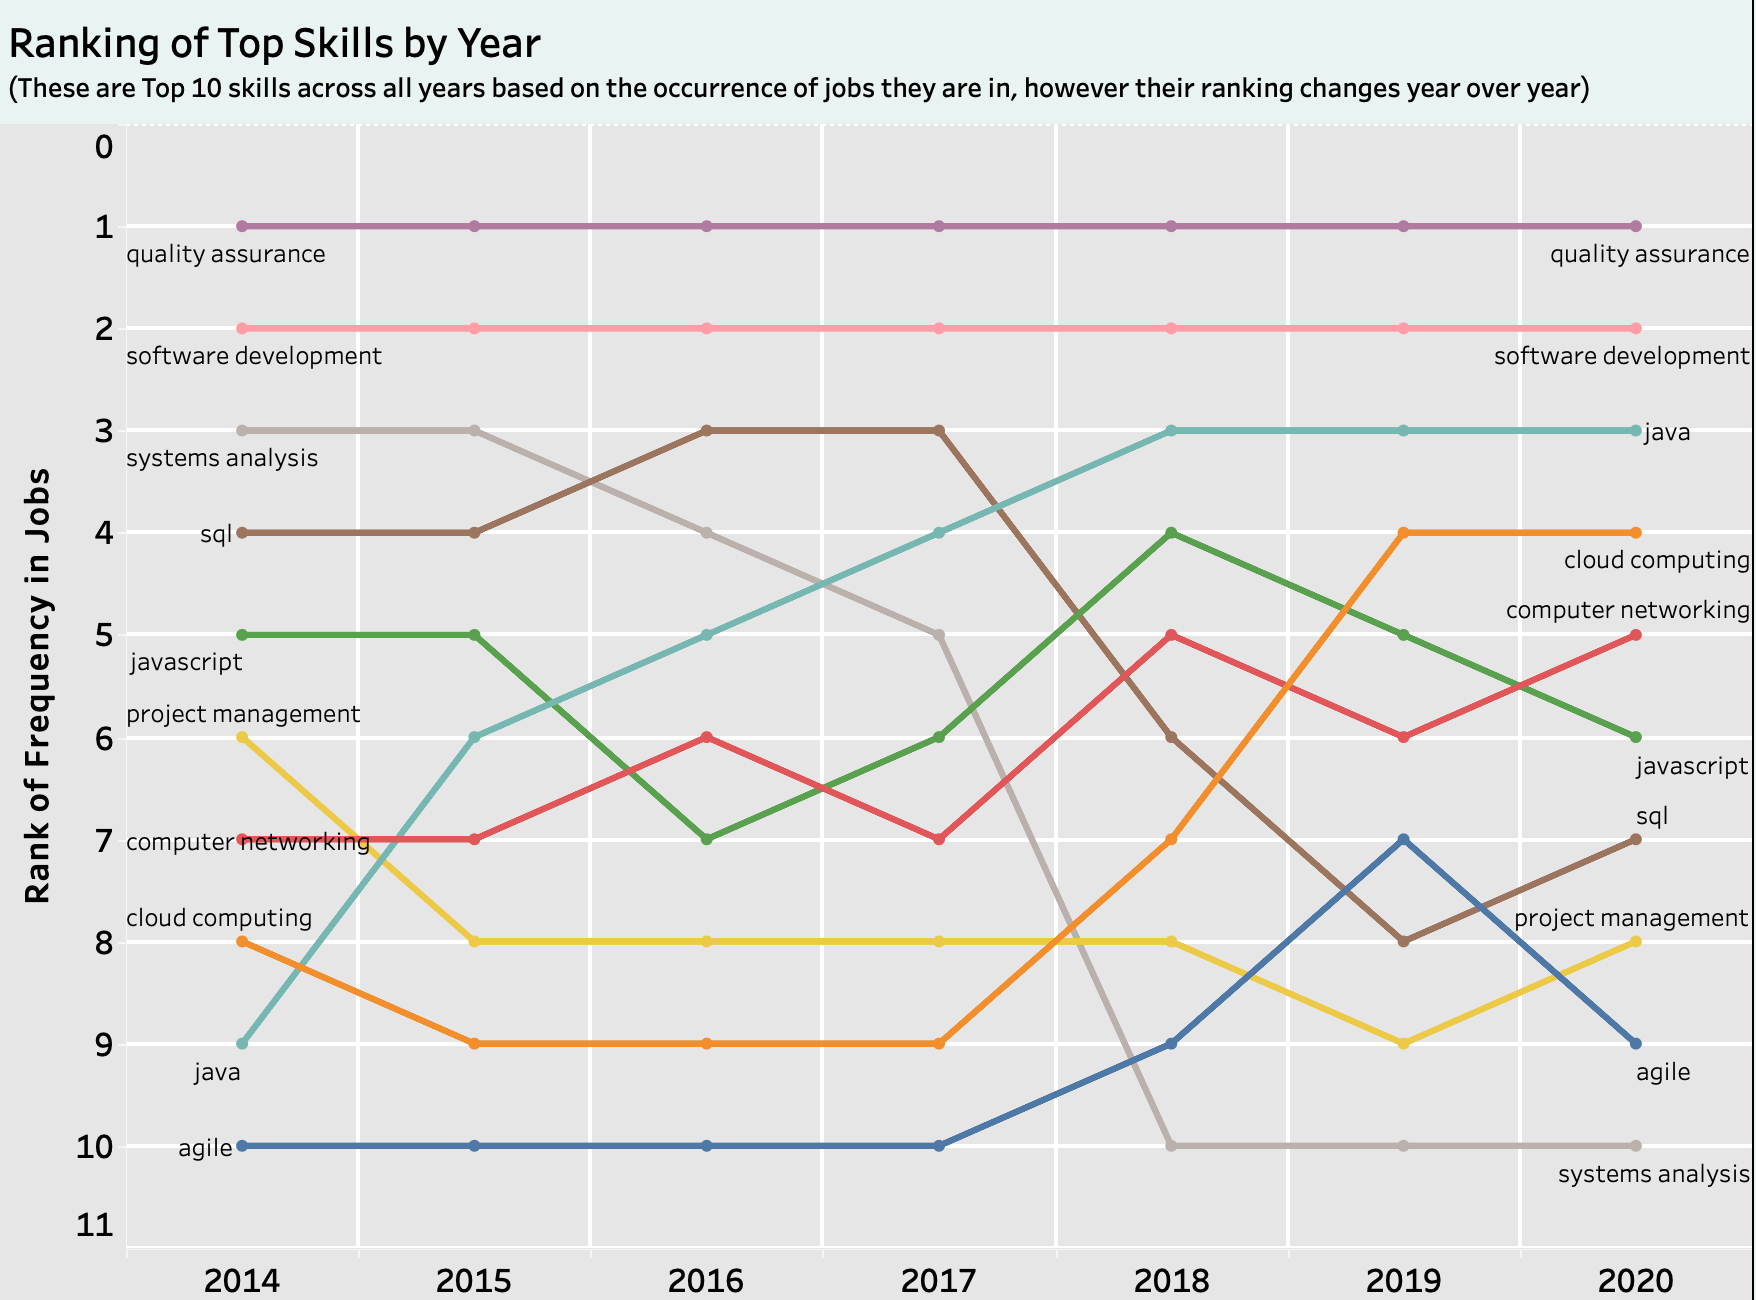
\includegraphics[width=\linewidth]{./photos/top10 ranking.png}
	\end{center}
	\caption{Skill 'trendiness' throughout the years}
	\label{trending}
\end{figure}
Next, let us take a look at the clustering results. 
\subsection{Clustering skill set}
The Following are  most frequent skills belong to each (total 10) cluster:
{\tiny
	\begin{itemize}
	\item Cluster 0
\subitem	sap	
\subitem	sap fi	
\subitem	sap fico	
\subitem	sap grc	
\subitem	sap mm
\subitem	sap pp	
	\item Cluster 1
\subitem	data warehouse	
\subitem	database
\subitem	etl	
\subitem	microsoft sql server
\subitem	microsoft ssis	
\subitem	quality assurance	
\subitem	software developmen
\subitem	sql
	\item Cluster 2
\subitem	computer networking	
\subitem	cyber security	
\subitem	dod	
\subitem	firewall	
\subitem	information security	
\subitem	policies	
\subitem	quality assurance	
\subitem	security clearance	
	
		\item Cluster 3
\subitem	analytics	
\subitem	database	
\subitem	health care	
\subitem	marketing	
\subitem	oracle	
\subitem	quality assurance	
\subitem	recruiting	
\subitem	research	
\subitem	software development	
\subitem	training	
		
			\item Cluster 4
\subitem	amazon web services	
\subitem	automation	
\subitem	cloud computing	
\subitem	computer networking	
\subitem	java	
\subitem	microsoft windows azure	
\subitem	python	
\subitem	quality assurance	
\subitem	sales	
\subitem	salesforce.com	
\subitem	software development	
			
				\item Cluster 5
\subitem	angularjs	
\subitem	cascading style sheets	
\subitem	html	
\subitem	html5	
\subitem	javascript	
\subitem	php	
\subitem	quality assurance	
\subitem	react.js	
\subitem	software development	
\subitem	ui	
\subitem	web development	
				
					\item Cluster 6
\subitem	brand	
\subitem	business development	
\subitem	customer relationship management	
\subitem	marketing	
\subitem	microsoft windows	
\subitem	quality assurance	
\subitem	recruiting	
\subitem	sales	
\subitem	salesforce.com	
\subitem	social media	
					
						\item Cluster 7
\subitem cisco	
\subitem	cisco certifications	
\subitem computer hardware	
\subitem	computer networking	
\subitem	microsoft windows	
\subitem	quality assurance	
\subitem	switches	
\subitem	technical support	
						
							\item Cluster 8
\subitem	agile	
\subitem	budget	
\subitem	it service management	
\subitem	planning	
\subitem	program management	
\subitem	project management	
\subitem	project planning	
\subitem	quality assurance	
\subitem	recruiting	
\subitem	training	
							
								\item Cluster 9
\subitem	.net	
\subitem	agile	
\subitem	automated testing	
\subitem	automation	
\subitem	c $\#$	
\subitem	java	
\subitem	quality assurance	
\subitem	software development	
\subitem	software engineering	
\subitem	sql	
								
								
\end{itemize}

}
We can easily guess that cluster 0 is SAP related, 1 is database. 2 is cyber-security, 4 is marketing, 5 is web developer, 7 computer is hardware, 8 is project management, 9 is software engineering.\\
Only cluster 3(health-tech) and 6 (Fin-tech) are a bit hard to define. Overall results for unsupervised learning is beyond our early expectation.
\section{Applications}
%How can the knowledge gained be applied?
There are infinite fields that our knowledge gain from this project be applied to. First, is the bigger picture of technology demand in  the US. For any recruiting company, the huge demand of particular job titles are the first thing they should pay attention to, since it is consider the 21st century capital, and need to competed for.\\
 Second is for job market on which skill-sets are in need so that job-seekers can have a better vision. Words like `A.I.' and `Machine learning' are too vague to be focused on, while skill-set from our cluster study shows that:\\
Third, there can be a better job category mapping within the knowledge gained, how and why certain jobs should be labeled as the same title with text clustering and Fuzzy matching. 
Many applications can be achieved with the future work on the same topic, due to the time limit for this project, we will sketch out the big picture for the future study in the next section. 
\section{Future work}
\subsection{Knowledge Graph}
'A knowledge graph, also known as a semantic network, represents a network of real-world entities—i.e. objects, events, situations, or concepts—and illustrates the relationship between them. This information is usually stored in a graph database and visualized as a graph structure, prompting the term knowledge “graph.'\footnote{IBM blog} Many web companies has their own graph base. For example, Google\footnote{\url{https://en.wikipedia.org/wiki/Google_Knowledge_Graph}} uses it to enhance search engine results with information gathered from a variety of sources. We can absolutely do the same for  technologist skills.\\
Figure \ref{connect} show the over all skill set connection training from the skill-set, we can definitely see the connection between each skill, and that is a 'gold mine' by itself, from this 'mine', we can easily map out the skill set for each job so that to find the 'shortest path' between each skill, e.g.: if a job is looking for a JAVA programmer, we can visualize a C++ person's resume, and see it is a good fit if not enough talent is found around that area. Figure \ref{directgraph} is a good demonstration on how close some skill with eachother. 
\subsection{Supply and demand of talent}
At Dice, we have almost all the tech job posts along with candidates' profile, and yet we do not have a good study on supply side of the market, if by mining with geo-location data, we can map out the talent pool around certain title demand, e.g.: if a company in Wyoming is looking for a particular skill set job and our database show no candidate in that area, we can recommend the profile close to that zip code, with the same or similar skill, a win-win situation for both.
\begin{figure}[h]
	\begin{center}
		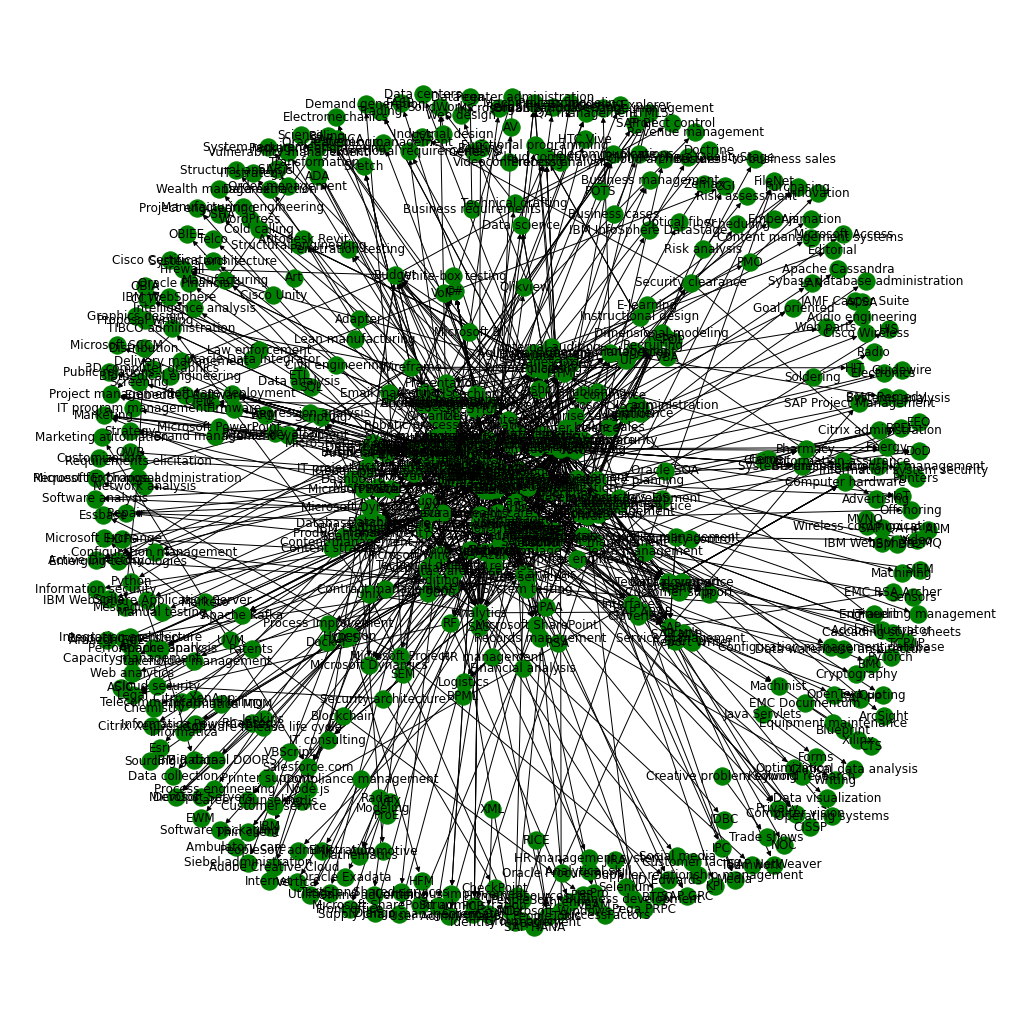
\includegraphics[width=\linewidth]{./photos/knowlegegraphsmall.png}
	\end{center}
	\caption{Overall connection of skillsets}
	\label{connect}
\end{figure}
\begin{figure}[h]
	\begin{center}
		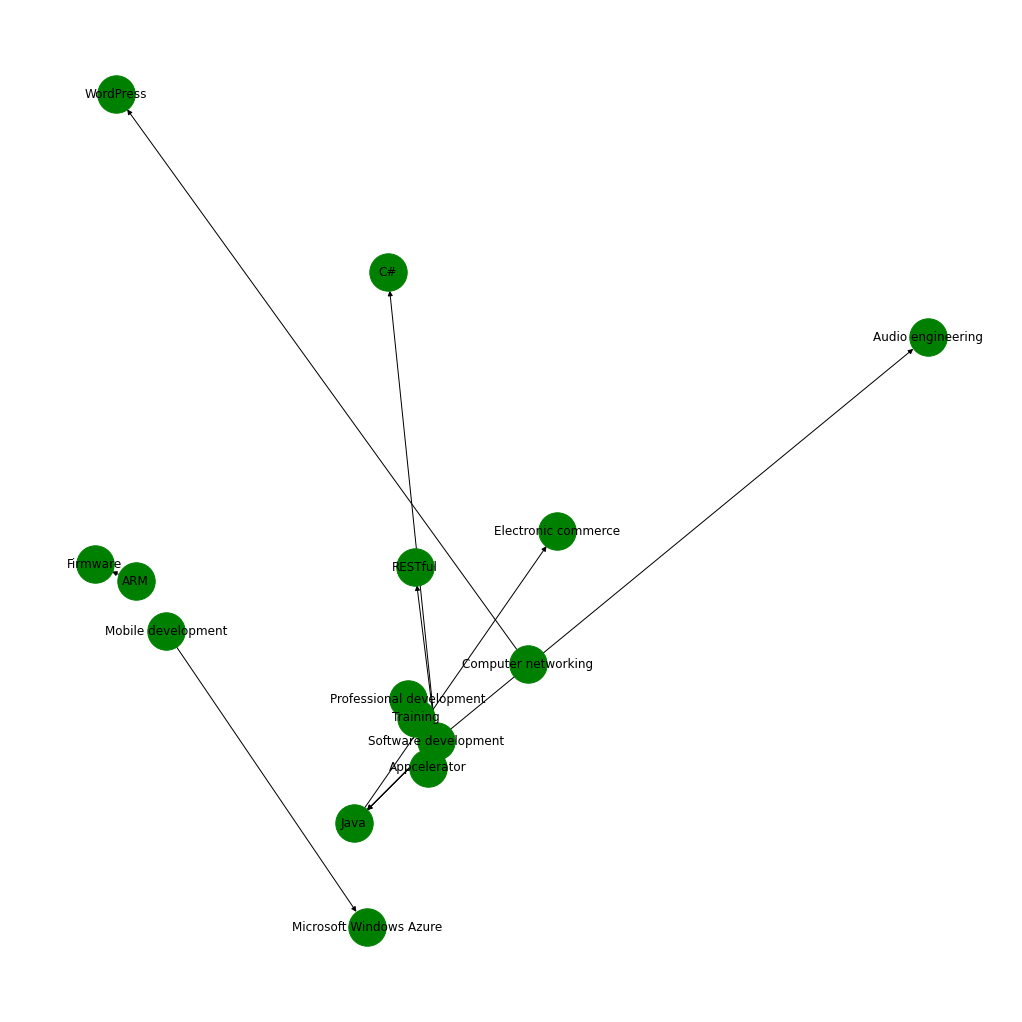
\includegraphics[width=\linewidth]{./photos/knowledgearrow2.png}
	\end{center}
	\caption{Directed graph between certain skill.}
	\label{directgraph}
\end{figure}
\subsection{Semi-supervised clustering}
As we see in Figure \ref{elbow}, there is not a definite cluster number that satisfies a good classification, and by introducing a semi supervised learning cluster may give us a satisfying result. As shown in Table \ref{titlemapping}, we can perhaps fine tune the clusters by first label some of the titles, so that the other ones can 'follow' the lead by learning the similar skill. 
\begin{table}[h!]
	\caption{job title mapping}
	\label{titlemapping}
	\resizebox{\columnwidth}{!}
	{%
		
		\begin{tabular}{lllll}
			\hline
			{} & 2018 SOC Code &                                   2018 SOC Title &    2018 SOC Direct Match Title &                      Job\_Title \\
			\hline
			0  &       15-1211 &                        Computer Systems Analysts &    Information Systems Analyst &    Information Systems Analyst \\
			1  &       15-1211 &                        Computer Systems Analysts &              Systems Architect &              Systems Architect \\
			2  &       15-1212 &                    Information Security Analysts &       Network Security Analyst &       Network Security Analyst \\
			3  &       15-1231 &             Computer Network Support Specialists &     Network Support Technician &     Network Support Technician \\
			4  &       15-1231 &             Computer Network Support Specialists &             Network Technician &             Network Technician \\
			5  &       15-1232 &                Computer User Support Specialists &          IT Support Specialist &          IT Support Specialist \\
			6  &       15-1241 &                      Computer Network Architects &               Network Engineer &               Network Engineer \\
			7  &       15-1243 &                              Database Architects &                 Data Architect &                 Data Architect \\
			8  &       15-1243 &                              Database Architects &    Data Integration Specialist &    Data Integration Specialist \\
			9  &       15-1243 &                              Database Architects &             Database Developer &             Database Developer \\
			10 &       15-1244 &      Network and Computer Systems Administrators &              LAN Administrator &              LAN Administrator \\
			11 &       15-1244 &      Network and Computer Systems Administrators &                Network Analyst &                Network Analyst \\
			12 &       15-1244 &      Network and Computer Systems Administrators &  Network Systems Administrator &  Network Systems Administrator \\
			13 &       15-1252 &                              Software Developers &      Software Systems Engineer &      Software Systems Engineer \\
			14 &       15-1253 &  Software Quality Assurance Analysts and Testers &      Software Quality Engineer &      Software Quality Engineer \\
			15 &       15-1254 &                                   Web Developers &                  Web Architect &                  Web Architect \\
			16 &       15-1254 &                                   Web Developers &                  Web Developer &                  Web Developer \\
			17 &       15-1255 &              Web and Digital Interface Designers &               Digital Designer &               Digital Designer \\
			18 &       15-1255 &              Web and Digital Interface Designers &         Web Content Specialist &         Web Content Specialist \\
			19 &       15-2031 &                     Operations Research Analysts &             Operations Analyst &             Operations Analyst \\
			20 &       15-2041 &                                    Statisticians &                Biostatistician &                Biostatistician \\
			21 &       15-2051 &                                  Data Scientists &   Data Visualization Developer &   Data Visualization Developer \\
			\hline
		\end{tabular}
		
	}
\end{table}
\subsection{Skill-sets Prediction}
One cool feature of time-series data is to predict using regression, yet out data collection failed at obtaining the recent H1b data to be able  study the growth rate of each skill set, in order to predict the future popular skill, this will help a company who focus on employee training to start the right path early in the game, it would also help a candidate to navigate his/her tech journal by betting on the right road map. 
\section{Conclusion}
In this project, we study the mining of US technologist data by combining US department of labor data along with web scraped H1b data set, after the introduction of word tagging to get skill set data, we clean and analyze the processed and joined data to later clustering the job skill data set. Since there is no clear technologist mining or analysis report online, our objective is to fill the blank page with knowledge of technologist's trench in the US studying  time series and Geo data. Our study shows that on top of tech talent demand in US are on the rise, is cloud engineering and project management skills will be in huge demand, while SQL and system analysis are in decline. Java still grows strong as python has not yet replace its spot, and Software developers should not worry that data scientists or ML engineers will make their job obsolete. \\
Our study's limitation is the availability of  lasted H1b data set along with non guidance on job title mapping table. In the first case: we are not able to do a deep time series analysis and prediction, in the latter, we do not have optimal clustering number for the unsupervised learning. 
We are looking forward to the future development of this topic with a better data set collection, the study of each topic can be its own project: Knowledge graph for each skill set, supply and demand of each job tile in the US hiring market, semi-supervised clustering with title mapping, and dynamic prediction for each skill and title.
\newpage 
\section*{Bonus material: Visualization}
We used Tableau\footnote{\url{https://public.tableau.com/app/profile/abulitibu.tuguluke/viz/H1BApplicationsv2/H1BJobs?publish=yes}} for our final visualization for this project. It contains  the following interaction information:\begin{enumerate}
\item A US map with H1b filtered by state and year.
\item Base salary distributing of most popular jobs filtered by state and year. 
\item Time series of skill ranking over year.
\item Most frequent skills by 10 clusters.  
\end{enumerate}

%Visualization of results (and/or link to interactive site to view or link to a video
%demonstrating the interactive site)






